\section{ConvTranspose}
Conv1DTranspose: 1 boyutlu transpoz konvolüsyon işlemi uygulamak için kullanılır. Giriş verileri üzerinde belirli bir pencere boyutunda kaydırılan bir filtre uygular. Conv1D katmanı giriş verisinin boyutunu azaltmak için kullanılırken, Conv1DTranspose katmanı giriş verisinin boyutunu artırmak için kullanılır.

\begin{figure}[h]
    \centering
    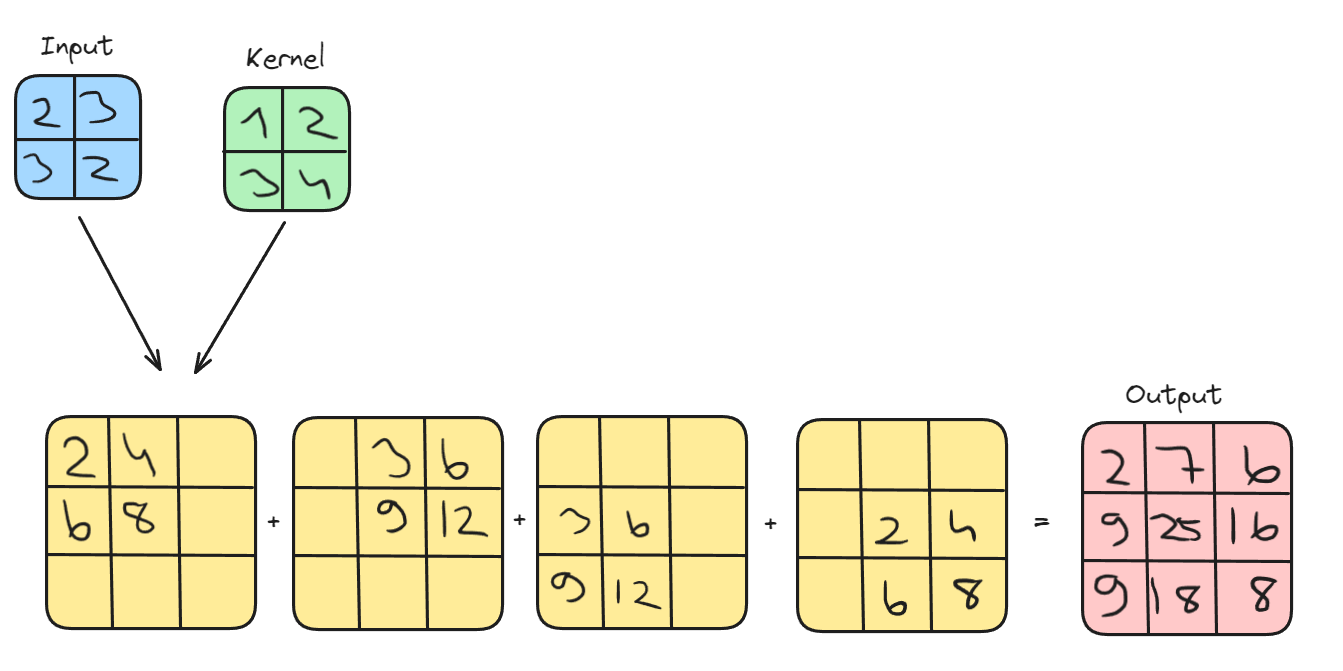
\includegraphics[width=0.7\textwidth]{images/conv_transpose_layer.png}
    \caption{De-Konvolüsyon katmanı.}
    \label{fig:enter-label}
\end{figure}

\subsubsection{Hiperparametreler}
\begin{table}[h]
\centering
{\scriptsize\renewcommand{\arraystretch}{0.4}
{\resizebox*{\linewidth}{0.2\textwidth}{
\begin{tabular}{|p{2cm}|p{6cm}|}
\hline
Parametre & Açıklama \\ \hline
filters & Çıkış uzayının boyutu. \\ \hline
kernel\_size & Filtre boyutu. \\ \hline
stride & Kaydırma adımı \\ \hline
padding & Giriş boyutunu ayarlamak için kullanılcak yöntem. \\ \hline
activation & Aktivasyon fonksiyonu. \\ \hline

\end{tabular}
}}}
\end{table}

\newpage